\documentclass[times,specification,annotation]{style/itmo-student-thesis/itmo-student-thesis}

\usepackage{icomma}
\usepackage{tabularx}

\usepackage{adjustbox}

\usepackage{tikz}
\usetikzlibrary{arrows}
\usepackage{tikz-qtree}
\usepackage{circuitikz}
\usepackage{pdfpages}

\usepackage{filecontents}
\begin{filecontents}{bachelor-thesis.bib}
@article{korneev-elizarov-pcms,
  title={Автоматическое тестирование решений на соревнованиях по программированию},
  author={Корнеев, ГА and Елизаров, РА},
  journal={Телекоммуникации и информатизация образования},
  number={1},
  pages={61--73},
  year={2003}
}
@book{stone1987program,
  title={Program construction},
  author={Stone, Richard Gary and Cooke, Derek John},
  number={22},
  year={1987},
  publisher={Cambridge University Press}
}
@book{mitchell2003concepts,
  title={Concepts in programming languages},
  author={Mitchell, John C and Apt, Krzysztof},
  year={2003},
  publisher={Cambridge University Press}
}
@online{competative-prog-wiki,
    year        = {2023},
    title       = {Competitive programming},
    url         = {https://en.wikipedia.org/w/index.php?title=Competitive_programming&oldid=1145645404},
    year        = {2023},
    langid      = {english}
}
@online{darkcyan-polygon-tutorial,
    year        = {2022},
    title       = {Polygon.Codeforces Tutorial - A Guide to Problem Preparation [Part 1]},
    author      = {Tran Quang Loc},
    url         = {https://quangloc99.github.io/2022/03/08/polygon-codeforces-tutorial.html},
    year        = {2022},
    langid      = {english}
}
@online{codeforces-rules,
    year        = {2012},
    title       = {Правила соревнований Codeforces},
    author      = {Мирзаянов, МР},
    url         = {https://codeforces.com/blog/entry/4088},
    year        = {2012},
    langid      = {russian}
}
@online{nerc-rules,
    year        = {2023},
    title       = {ICPC Northern Eurasia Regional Contest Rules},
    url         = {https://neerc.ifmo.ru/information/contest-rules.html},
    year        = {2023},
    langid      = {english}
}
@online{roi-regionals-requirements,
    year        = {2022},
    title       = {Требования к организации и проведению регионального этапа Всероссийской олимпиады школьников в 2022/2023 учебном году по информатике},
    url         = {https://edsoo.ru/download/1076/?hash=33c893065154553c8704a8a0cbe9860e},
    year        = {2022},
    langid      = {russian}
}
@online{ioi-rules,
    year        = {2022},
    title       = {IOI Competition Rules},
    url         = {https://ioi2022.id/competition-rules/},
    year        = {2022},
    langid      = {english}
}
@online{cf-graders,
    year        = {2019},
    author      = {Мирзаянов, МР},
    title       = {Polygon: расширенные свойства ресурсов (грейдеры)},
    url         = {https://codeforces.com/blog/entry/66916},
    year        = {2019},
    langid      = {english}
}
@article{parr2013definitive,
  title={The definitive ANTLR 4 reference},
  author={Parr, Terence},
  journal={The Definitive ANTLR 4 Reference},
  pages={1--326},
  year={2013},
  publisher={The Pragmatic Bookshelf}
}
@article{aho-compilers,
  title={Компиляторы: принципы, технологии и инструментарий},
  author={Ахо, А and Лам, М and Сети, Рави and Ульман, Дж},
  journal={М.: Вильямс},
  volume={1},
  pages={257},
  year={2008}
}
@book{design-patterns,
  title={Паттерны объектно-ориентированного проектирования},
  author={Эрих, Г. and Ричард, Х. and Роберт, Д. and Джон, В.},
  year={2020},
  publisher={"Издательский дом ""Питер"""}
}
@online{cf-testlib,
    year        = {2015},
    author      = {Мирзаянов, МР},
    title       = {Коротко о testlib.h},
    url         = {https://codeforces.com/testlib},
    year        = {2015},
    langid      = {russian}
}
@book{cppbook,
  title={Язык программирования C++},
  author={Страуструп, Б.},
  year={2011},
  publisher={Бином}
}
@online{cppcin,
    year        = {2021},
    title       = {std::cin, std::wcin},
    url         = {https://en.cppreference.com/w/cpp/io/cin},
    year        = {2021},
    langid      = {english}
}
@online{javascanner,
    year        = {2022},
    title       = {Class Scanner (Java SE 19)},
    url         = {https://download.java.net/java/early_access/panama/docs/api/java.base/java/util/Scanner.html},
    year        = {2022},
    langid      = {english}
}
@book{laurent2001programming,
  title={Programming Web Services with XML-RPC: Creating Web Application Gateways},
  author={Laurent, Simon St and Johnston, Joe and Wilder-James, Edd and Winer, Dave},
  year={2001},
  publisher={" O'Reilly Media, Inc."}
}
@online{protobufdocs,
    year        = {2023},
    title       = {Protocol Buffers},
    url         = {https://protobuf.dev/},
    year        = {2023},
    langid      = {english}
}
\end{filecontents}

\addbibresource{bachelor-thesis.bib}

\begin{document}

\studygroup{M34371}
\title{Автоматизация построения программных компонентов при подготовке задач по спортивному программированию}
\author{Назаров Георгий Дмитриевич}{Назаров Г.Д.}
\supervisor{Корнеев Георгий Александрович}{Корнеев Г.А.}{доцент, к.т.н.}{доцент факультета информационных технологий и программирования}
\publishyear{2023}
\startdate{10}{апреля}{2023}
\finishdate{15}{мая}{2023}

\addconsultant{Мирзаянов М.Р.}{без степени, без звания}

\secretary{Штумпф С.А.}

\technicalspec{
    Требуется разработать систему, автоматизирующую процесс построения программных компонентов при подготовке (разработке) задач по спортивному программированию, в том числе:

    1. Спроектировать специальный язык описания входных и выходных данных, требуемых в задаче по спортивному программированию.

    2. Реализовать систему кодогенерации, которая, на основании описания входных и выходных данных, будет генерировать исходный код программных компонентов задачи, в том числе:

    2.1. Программы, проверяющей ответ участника (чекера);

    2.2. Программы, проверяющей корректность входных данных (валидатора);

    2.3. Компонентов ввода-вывода пользовательских решений задачи (грейдеров).

    3. Внедрить полученную систему в сервис подготовки задач по спортивному программированию «Polygon».
}

\plannedcontents{?}

\plannedsources{\begin{enumerate}
    \item ?
\end{enumerate}}

\researchaim{?}

\researchtargets{\begin{enumerate}
    \item ?
\end{enumerate}}

\addadvancedsoftware{?}{?}

\researchsummary{?}

\researchfunding{?}

\researchpublications{?}

% \maketitle{Бакалавр}

\includepdf{include/title.pdf}
\includepdf[pages={1-2}]{include/abstract.pdf}
\includepdf[pages={1-2}]{include/annotation.pdf}

%% Ставим номер страницы сверху по центру
\newcommand{\TheOnlyTruePageStyle}{fancy}
\pagestyle{\TheOnlyTruePageStyle}
\renewcommand{\headrulewidth}{0pt}
\renewcommand{\footrulewidth}{0pt}
\lhead{}
\chead{\thepage}
\rhead{}
\lfoot{}
\cfoot{}
\rfoot{}
\addtolength{\voffset}{3mm}
\addtolength{\headsep}{-3mm}

\setcounter{page}{4}
% Выключаем переносы в оглавлении
\pretocmd{\tableofcontents}{\begingroup\banhyphens}{}{}
\apptocmd{\tableofcontents}{\endgroup}{}{}

\tableofcontents

\startprefacepage

Соревнования по спортивному программированию проходят с использованием автоматизированных систем тестирования~\cite{korneev-elizarov-pcms}, например, PCMS2, Ejudge, Яндекс.Контест, Codeforces. Участники отсылают на проверку исходный код программы-решения, которая автоматически проверяется на наборе тестов~\cite{competative-prog-wiki}.

Для того, чтобы задачу по спортивному программированию можно было использовать в автоматизированной тестирующей системе, авторы задачи должны предварительно подготовить <<пакет>> задачи, состоящий из условий задачи, тестов и набора программ, участвующих в процессе тестирования~\cite{darkcyan-polygon-tutorial}. Подготовка каждой задачи~--- трудоемкий ручной процесс, легко подверженный ошибкам.

В работе реализована система кодогенерации, позволяющая частично автоматизировать процесс подготовки задачи путем генерации некоторых программных компонентов задачи. Полученное решение внедрено в сервис для подготовки задач по спортивному программированию <<Polygon>>.

В главе 1 подробно описана предметная область~--- процесс соревнований по спортивному программированию, в том числе их подготовка. В главе 2 описывается специальный язык описания входных и выходных данных. В главе 3 изложены детали реализации языка. В главе 4 описывается процесс генерации исходного кода программных компонентов задач по спортивному программированию и интеграция решения в <<Polygon>>.

\chapter{Обзор предметной области}

В данной главе приводятся описания существующего процесса подготовки задач по спортивному программированию и процесса участия в соревнованиях по спортивному программированию с точки зрения участника. В дальнейшей работе будут использоваться термины и определения, вводимые в этой главе.

\section{Соревнования с точки зрения участников}

На соревнованиях по спортивному программированию участникам предлагается к решению упорядоченный набор задач. За ограниченное количество времени участники должны решить как можно больше задач и как можно точнее (определение <<точности>> зависит от правил конкретного соревнования).

К каждой задаче прилагается условие задачи~--- текстовое человекочитаемое описание требований к решению участника. Решением участника является исходный код на одном из доступных в автоматизированной системе тестирования языков программирования. Решение задачи может содержать, в зависимости от правил соревнования, как весь исходный код программы-решения, так и его часть~--- реализацию заданного в условии задачи интерфейса или функции с необходимой сигнатурой.

После проверки решения, участнику сообщается вердикт проверки~--- строка с информацией о корректности решения, возможно, содержащая дополнительную информацию, например, номер теста, на котором решение участника выдало неправильный ответ~\cite{codeforces-rules},~\cite{nerc-rules}.

\section{Процесс тестирования}

После получения решения участника автоматизированная тестирующая система выполняет его обработку, состоящую из следующих основных шагов~\cite{roi-regionals-requirements}:

\begin{enumerate}
    \item Компиляция решения участника;
    \item Компоновка (линковка) решения участника с компонентами задачи (при необходимости);
    \item Генерация наборов входных данных (для генерируемых тестов);
    \item Валидация входных данных на соответствие условию задачи;
    \item Запуск исполняемого файла с решением на наборе тестов (входных данных);
    \item Запуск программы проверки ответа участника на каждом из тестов и ответов программы-решения;
\end{enumerate}

В зависимости от правил соревнования шагов может быть больше. Об ошибке на любом из шагов сообщается участнику.

\section{Подготовка задач}

Чтобы задачу можно было использовать в автоматизированной тестирующей системе, авторы задачи должны подготовить следующие компоненты задачи~\cite{darkcyan-polygon-tutorial}:

\begin{enumerate}
    \item Условия задачи, возможно, на нескольких языках;
    \item Валидатор (от англ. \textit{validator})~--- программу, принимающую на вход произвольный текстовый файл и выдающую вердикт, может ли быть этот файл использован в качестве теста в конкретной задачи. Валидатор должен проверять структуру файла и соответствие значений переменных ограничениям из условия;
    \item Чекер (от англ. \textit{checker})~--- программу, принимающую на вход тест, ответ программы участника и ответ жюри (авторского решения), и выдающая вердикт о корректности ответа участника. Чекер дожен проверять выполнение в ответе ограничений из условия задачи.
    \item Тесты (входные данные)~--- текстовые файлы, которые будут подаваться на вход решению участника. Могут быть заданы вручную или генерироваться во время тестирования;
    \item Генераторы~--- программы, принимающие в аргументах командной строки параметры, на основании которых генерируют (выводят) тест или набор тестов;
    \item Решение жюри (авторское решение)~--- исходный код эталонного решения задачи. Используется для получения эталонных ответов при запуске чекера;
\end{enumerate}

На некоторых соревнованиях от участников не требуется полная реализация решения, а только лишь его части~--- функции с заданной сигнатурой или интерфейса. (Подобные правила применяются, например, на IOI~--- международной олимпиаде по информатике~\cite{ioi-rules}). В таком случае авторам задачи так же необходимо подготовить грейдеры (от англ. \textit{grader}, <<оценщик>>)~--- часть исходного кода решения, которая будет скомпонована (слинкована) с решением участника. Исходный код грейдеров должен обязательно содержать точку входа программы и реализацию ввода-вывода, специфичную для задачи. Опционально, грейдеры могут выполнять дополнительные действия перед передачей управления коду участника или после окончания выполнения кода участника. Грейдеры должны быть написаны на каждом из доступных участнику языков программирования~\cite{cf-graders}.

Рассмотрим подробнее, что представляют собой тесты (входные данные) и выходные данные в задачах по спортивному программированию. Как было сказано выше, это текстовые файлы с определенной автором задачи структурой. В условии задачи описываются переменные и ограничения на них~--- тесты, в свою очередь, состоят из значений этих переменных, причем значения разделены пробелами и переводами строк в порядке, определенном автором задачи (и указанном в условии). Выходные данные так же состоят из значений переменных, разделенных в установленном порядке пробелами и переводами строк.

\section{Примеры программных компонентов задачи}

Рассмотрим подробнее программные компоненты на примере задачи <<A~+~B>>.

На листинге~\ref{a-plus-b-validator} приведен исходный код валидатора. В нем считывается два целочисленных значения в интервале от $-1000$ до $1000$, разделенных одним пробелом. Затем ожидается перевод строки и конец файла теста.

\begin{lstlisting}[float=!h,caption={Пример валидатора},label={a-plus-b-validator},language=c++]
#include "testlib.h"

int main(int argc, char *argv[])
{
    registerValidation(argc, argv);
    inf.readInt(-1000, 1000, "a");
    inf.readSpace();
    inf.readInt(-1000, 1000, "b");
    inf.readEoln();
    inf.readEof();
    return 0;
}
\end{lstlisting}

На листинге~\ref{a-plus-b-checker} приведен исходный код чекера. В нем считывается одно целочисленное значение в интервале от $-2000$ до $2000$ два раза: сначала ответ участника, затем ответ жюри (вывод авторского решения). Если ответы совпали, участник получает вердикт <<Правильный ответ>>, в противном случае <<Неправильный ответ>>, на соответствующем тесте.

\begin{lstlisting}[float=!h,caption={Пример чекера},label={a-plus-b-checker},language=c++]
#include "testlib.h"

int readAns(InStream& stream)
{
    return stream.readInt(-2000, 2000, "sum");
}

int main(int argc, char *argv[])
{
    registerTestlibCmd(argc, argv);
    int participant = readAns(ouf);
    int jury = readAns(ans);
    if (participant != jury)
        quitf(_wa, "Wrong answer");
    else
        quitf(_ok, "Ok");
}
\end{lstlisting}

Тесты могут быть сгенерированы программно. На листинге~\ref{a-plus-b-generator} приведен исходный код генератора случайных тестов. Принимает на вход единственный аргумент командной строки~--- ограничение на абсолютную величину генерируемых значений. Два случайных значения выводятся в стандартный поток вывода через пробел, затем следует перевод строки.

\begin{lstlisting}[float=!h,caption={Пример генератора},label={a-plus-b-generator},language=c++]
#include <iostream>
#include "testlib.h"
 
int main(int argc, char* argv[]) {
    registerGen(argc, argv, 1);
 
    int N = opt<int>(1);
    std::cout << rnd.next(-N, N) << ' ';
    std::cout << rnd.next(-N, N) << std::endl;
    return 0;
}
\end{lstlisting}

Грейдеры являются написанной жюри (автором задачи) частью исходного кода, который будет скомпонован с реализацией участника для получения полного исполняемого файла с решением. Грейдеры должны быть написаны на всех, доступных для использования участниками, языках программирования. 

На листинге~\ref{a-plus-b-grader-cpp} приведен исходный код грейдера для языка программирования C++. Грейдеры для C++ обычно состоят из двух файлов: заголовочного и главного. Заголовочный файл, импортируемый кодом участника, содержит определение требуемых к реализации функций и функций, написанных жюри, доступных для использования участником. Главный файл содержит точку входа (функцию \texttt{main()}, с которой будет начато исполнение) и код, считывающий входные данные из стандартного потока ввода и выводящий ответ, полученный вызовом пользовательской реализации, в стандартный поток вывода.

\begin{lstlisting}[float=!h,caption={Пример грейдера для языка C++},label={a-plus-b-grader-cpp},language=c++]
// aplusb.h

int sum_ab(int a, int b);

// grader.cpp

#include <iostream>
#include "aplusb.h"
 
int main() {
    int a, b;
    std::cin >> a >> b;
    std::cout << sum_ab(a, b) << std::endl;
    return 0;
}
\end{lstlisting}

На листинге~\ref{a-plus-b-grader-py} приведен исходный код грейдера для языка программирования Python. Так как Python~--- интерпретируемый язык программирования, понятие линковки для него не определено, поэтому грейдер напрямую импортирует и вызывает решение участника. Блок кода в середине содержит проверку версии языка, чтобы грейдер мог работать как на Python 2, так и на Python 3.

\begin{lstlisting}[float=!h,caption={Пример грейдера для языка Python},label={a-plus-b-grader-py},language=python]
import solution
import sys

if sys.version_info[0] < 3:
    _input = raw_input
else:
    _input = input
 
a, b = map(int, _input().split())
print(solution.sum_ab(a, b))
\end{lstlisting}

\section{Цели и задачи ВКР}

В предыдущих пунктах показано, что для подготовки даже простых задач по спортивному программированию авторам задачи необходимо проделать существенную работу, написав исходный код для, как минимум, трёх программных компонентов~--- валидатора, чекера и генератора, при этом генераторов может быть много, для того, чтобы сгенерировать как можно более разнообразные тесты. При этом, в случае, если задача подразумевает наличие грейдеров, объем исходного кода, необходимого к написанию, становится пропорциональным количеству поддерживаемых тестирующей системой языков программирования.

% Задание на ВКР

Основная цель данной выпускной квалификационной работы~--- разработка системы, автоматизирующей процесс реализации программных компонентов при подготовке задач по спортивному программированию.

В ходе консультаций с авторами задач по спортивному программированию были выделены следующие задачи, решаемые в данной выпускной квалификационной работе:

\begin{enumerate}
    \item Необходимо спроектировать специальный язык описания входных и выходных данных, специфичных для задачи.
    \item Реализовать систему кодогенерации, которая будет принимать на вход описание входных и выходных данных, на основании которой будет частично сгенерирован исходный код валидатора, чекера и грейдеров.
    \item Внедрить реализованную систему в сервис подготовки задач по спортивному программированию <<Polygon>>.
\end{enumerate}

\chapter{Проектирование языка описания входных и выходных данных}

В этой главе формулируются требования к языку описания входных и выходных данных и описывается разработанный язык описания входных и выходных данных.

\section{Требования к языку описания}

В ходе консультаций с авторами задач по спортивному программированию были выделены следующие требования к возможностям языка описания:

\begin{enumerate}
    \item Должна быть возможность указывать название для каждой переменной. Это необходимо для генерации человекочитаемых сообщений об ошибках в валидаторе и чекере.
    \item Должна быть возможность указывать тип переменных, для корректной реализации ввода-вывода.
    \item Должна быть возможность описывать структуры~--- упорядоченный набор семантически связных переменных.
    \item Должна быть возможность указывать места перевода строк.
    \item Должна быть возможность задавать ограничения на переменные~--- для проверки корректности данных.
\end{enumerate}

Отдельно стоит отметить одно неформальное требование: язык описания должен иметь <<низкий порог входа>>. Иными словами, <<простые>> входные и выходные данные должны с его помощью описываться <<простыми>> конструкциями.

Так же для удобства последующей реализации было принято решение ограничить возможный язык описания классом $LL(1)$ контекстно-свободных грамматик.

\section{Язык описания входных и выходных данных}

Входные и выходные данных представляют собой текстовые файлы, содержимое которых удовлетворяет описанным в условии задачи ограничениям и формату. Разработанный язык описания представляет способ текстового машиночитаемого описания структуры входных и выходных данных, понятного человеку. Для построения лексического и синтаксического анализаторов языка описания был использован генератор нисходящих анализаторов для формальных языков \textit{ANTLR 4}~\cite{parr2013definitive}. Полная грамматика языка описания представлена в Приложении~\ref{appendix-antlr-grammar}.

Файл описания входных и выходных данных состоит из набора \textit{структур}~--- объявлений семантически объединенных переменных, идущих во входных или выходных данных в указанном в описании порядке. Переменные внутри структуры могут представлять собой значения, массивы или другие структуры.

Каждая структура опционально может иметь некоторое, возможно нулевое, количество \textit{параметров}~--- переменных или выражений, которые необходимы для ввода-вывода соответствующей структуры. Структуры могут содержать переменные, условные операторы и модификаторы ввода-вывода. Условные операторы используются для изменения набора переменных в структуре в зависимости от какого-либо условия~--- выражения, вычислимого из переменных с известным значением (то есть тех, которые будут к моменту ввода-вывода текущей структуры уже содержались в вводе или выводе). Модификаторы ввода-вывода используются для изменения разделителей между переменными и указания необходимого форматирования во входных и выходных данных.

Объявление переменной содержит название соответствующей переменной, её тип и, опционально, ограничение на эту переменную, представленное выражением, записанном на языке выражений, который будет рассмотрен позднее. Выражения в ограничениях должны иметь логический тип.

Подробное описание языковых конструкций будет рассмотрено позднее в данной работе.

\subsection{Лексика языка описания}

Листинг~\ref{appendix-lexer-src} содержит определения используемых в языке типов токенов (лексем)~--- неделимых синтаксических конструкций языка. Рассмотрим типы токенов подробнее.

Типы токенов \texttt{LINE\_COMMENT}, \texttt{COMMENT} и \texttt{WS} отвечают за комментарии и пробельные символы. Такие токены должны впоследствии игнорироваться синтаксическим анализатором, что указано директивой \texttt{-> skip} после них. Однострочные комментарии начинаются с символа <<\texttt{\#}>> и продолжаются до конца строки. Блоковые комментарии обрамляются последовательностями символов <<\texttt{/*}>> и <<\texttt{*/}>>.

Типы токенов \texttt{CHAR} и \texttt{STRING} отвечают за символьные и строковые константы соответственно.

Типы токенов \texttt{TRUE} и \texttt{FALSE} отвечают за логические константы <<истина>> и <<ложь>> соответственно.

Типы токенов \texttt{LOGICAL\_AND}, \texttt{LOGICAL\_OR} и \texttt{LOGICAL\_NOT} отвечают за операторы логической конъюнкции, дизъюнкции и отрицания. 

Типы токенов \texttt{BITWISE\_AND}, \texttt{BITWISE\_XOR} и \texttt{BITWISE\_NOT} отвечают за операции <<Побитовое И>>, <<Побитовое исключающее ИЛИ>> и <<Инверсия битов>>. Тип токена \texttt{PIPE} является неоднозначным, но, в том числе, отвечает за операцию <<Побитовое ИЛИ>>.

Типы токенов \texttt{EQUALS}, \texttt{NOT\_EQUALS}, \texttt{LESS\_EQUAL}, \texttt{GREATER\_EQUAL}, \texttt{LESS} и \texttt{GREATER} отвечают за операторы сравнения: равенство, неравенство, <<меньше или равно>>, <<больше или равно>>, <<меньше>> и <<больше>> соответственно.

Затем следует блок типов токенов, отвечающих за арифметические операции: \texttt{PLUS}, \texttt{MINUS}, \texttt{POW}, \texttt{MULTIPLICATION}, \texttt{DIVISION}, \texttt{MODULO}~--- сложение, вычитание, возведение в степень, умножение, деление и взятие остатка от деления (взятие по модулю) соответственно.

Тип токена \texttt{QUESTION} используется в тернарном условном операторе, как и многозначный \texttt{COLON}.

Тип токена \texttt{ASSIGN} используется в некоторых синтаксических конструкциях описания входных и выходных данных, семантически схожих с операцией присваивания значения переменной.

Тип токена \texttt{COMMA} используется в качестве разделителя аргументов функций и в семантически похожих конструкциях.

Тип токена \texttt{SEMICOLON} используется в качестве разделителя списка объявляемых переменных.

Типы токенов \texttt{LBRACE} и \texttt{RBRACE} используются для обозначения границ логического блока.

Типы токенов \texttt{LBRACKET} и \texttt{RBRACKET} используются в качестве обозначения индексации массивов и при определении массивов.

Типы токенов \texttt{LPAR} и \texttt{RPAR} используются для обозначения границ списка аргументов функций.

Затем следует блок типов токенов, являющихся зарезервированными словами языка описания входных и выходных данных. Это \texttt{SEP}, \texttt{EOLN\_MODIFIER}, \texttt{IF}, \texttt{ARRAY}, \texttt{OF} и \texttt{else}. Типы \texttt{IF} и \texttt{else} используются в условном операторе. Типы \texttt{SEP} и \texttt{EOLN\_MODIFIER} используются при указании разделителя между переменными во входных и выходных данных. Типы \texttt{ARRAY} и \texttt{OF} используются при объявлении массивов неименованных структур.

Затем следует составное определение типа токена \texttt{NUM\_VALUE}. Токены этого типа могут содержать целочисленные значения или числа с плавающей точкой (в том числе в экспоненциальном виде). Используя суффиксы можно явно указать тип, в который будет транслироваться токен при кодогенерации.

Тип токена \texttt{NAME} отвечает за идентификаторы. Для упрощения последующей кодогенерации, идентификаторы могут содержать только буквы латинского алфавита, арабские цифры и символы <<\texttt{\_}>>.

Как можно видеть из листинга~\ref{appendix-lexer-src}, почти все операторы позаимствованы из языка программирования C++, за исключением оператора возведения в степень, так как соответствующий оператор в C++ отсутствует. Это сделано чтобы авторы задач могли писать выражения на языке максимально приближенном к С++, на котором подготавливается подавляющее большинство задач по спортивному программированию. Далее так же будет показано, что приоритеты операторов так же идентичны таковым в языке программирования C++.

\subsection{Синтаксис языка описания}

Листинг~\ref{appendix-grammar-src} содержит формальную грамматику языка описания входных и выходных данных в формате ANTLR. Стартовым символом грамматики является нетерминал \texttt{ioMarkup}, раскрывающийся в список нетерминалов \texttt{namedStruct}~--- список определений структур.

Каждое определение структуры начинается с токена с типом \texttt{NAME}~--- названия соответствующей структуры. Названия структур должны быть уникальными и не совпадать с названиями встроенных типов. Затем следует необязательные параметры структуры (нетерминал \texttt{namedStructParameters}) и после них описание структуры (нетерминал \texttt{struct}).

Параметры структуры состоят из списка объявлений параметров (нетерминалы \texttt{parameterDeclaration}), разделенных запятыми, обрамленного круглыми скобками. Каждое объявление параметра состоит из имени параметра (\texttt{NAME}) и названия типа этого параметра, разделенных символом двоеточия.

Описание структуры состоит из списка элементов описания (нетерминалы \texttt{structItem}), обрамленного фигурными скобками. Элементами описания могут быть условные операторы (нетерминал \texttt{conditionalAlternative}), объявления переменных (нетерминал \texttt{variableDeclaration}) или модификаторы ввода-вывода (нетерминал \texttt{ioModifier}).

Объявления переменных состоят из названия переменной, затем следует символ двоеточия, после него пишется тип переменной (нетерминал \texttt{variableType}). Затем, опционально, следует символ вертикальной черты и ограничение на переменную, записанное на языке выражений (нетерминал \texttt{plExpression} из листинга~\ref{appendix-grammar-pl-src}). Завершается описание переменной символом точки с запятой.

Тип переменной задается следующим образом. Сначала записывается название типа (предопределенное или название объявленной автором задачи структуры), затем, опционально, следуют параметры структуры (нетерминал \texttt{namedTypeParameters}), состоящие из списка выражений, после чего, опционально, следуют одно или несколько деклараций массива (нетерминалы \texttt{arrayParameters}).

Декларации массива меняют тип переменной с одиночного на массив соответствующего типа. Декларация массива состоит из объявления переменной итерирования с указанием начального и конечного значений итерирования (нетерминал \texttt{arrayIterationRange}). Затем, через запятую, указывается разделитель переменных в массиве~--- строка, состоящая из пробелов или экранированных переводов строк (нетерминал \texttt{sepValue}).

Поддержана возможность определения массивов неименованных структур (массивов кортежей с именованными элементами). Для этого в качестве типа переменной указывается конструкция <<\texttt{array ... of}>> (нетерминал \texttt{arrayOfUnnamedStruct}), после которой следует описание структуры. Вместо двоеточия пишутся декларации массива.

\subsection{Синтаксис выражений}

Для записи выражений в декларациях массивов и ограничениях на переменные используется специальный синтаксис выражений, представленный ANTLR грамматикой в листинге~\ref{appendix-grammar-pl-src}. Стартовым нетерминалом является \texttt{plExpression}.

Нетерминал \texttt{plValue} отвечает за запись константных значений. Нетерминал \texttt{plVarBinding} отвечает за использование значения переменной в выражении. Операторы языка выражений и остальные нетерминалы представлены в таблице~\ref{pl-operators-priority}. Стартовым нетерминалом грамматики является \texttt{plExpression}.

Выражения записываются в виде, максимально приближенном к языку программирования C++, как к наиболее популярному языку программирования, использующегося при подготовке задач.

\subsection{Система типов}

Язык описания входных и выходных данных имеет встроенные целочисленные, строковые, символьные, логические типы и тип вещественных чисел с плавающей точкой. Полный список встроенных типов приведен в таблице~\ref{predefined-types}.

\begin{table}[!h]
\caption{Встроенные типы данных}\label{predefined-types}
\centering
\begin{tabular}{|*{3}{c|}}\hline
Тип & Описание & Пример\\\hline
\texttt{bool} & Логический тип & \texttt{true} \\\hline
\texttt{char} & Символьный тип & \texttt{'x'}\\\hline
\texttt{int32} & $32$-х битный целочисленный знаковый тип & \texttt{123} \\\hline
\texttt{uint32} & $32$-х битный целочисленный беззнаковый тип & \texttt{123u} \\\hline
\texttt{int64} & $64$-х битный целочисленный знаковый тип & \texttt{123l} \\\hline
\texttt{uint64} & $64$-х битный целочисленный беззнаковый тип & \texttt{123ul} \\\hline
\texttt{float32} & $32$-х битный тип чисел с плавающей точкой & \texttt{12.3f} \\\hline
\texttt{float64} & $64$-х битный тип чисел с плавающей точкой & \texttt{12.3} \\\hline
\texttt{string} & Строковый тип (массив символов) & \texttt{"abc"} \\\hline
\end{tabular}
\end{table}

Язык описания выходных и выходных данных поддерживает структуры данных~--- объявленные пользователем составные типы, состоящие из упорядоченного набора переменных других, возможно составных, типов. Пример структуры данных приведен на листинге~\ref{struct-example}.

\begin{lstlisting}[
    caption={Пример структуры},
    keywordstyle=\color{black},
    commentstyle=\color{black},
    stringstyle=\color{black},
    label={struct-example}
]
pair {
    a: int32;
    b: int32;
}
\end{lstlisting}

К любому типу переменной при объявлении может быть дописан суффикс, являющийся декларацией массива. Такая конструкция объявляет массив указанного типа.

\chapter{Реализация языка описания входных и выходных данных}

В этой главе описываются алгоритмы обработки языка описания входных и выходных данных, а так же реализация соответствующих алгоритмов.

\section{Обработка языка описания}

Был реализован инструмент, принимающий на вход описание входных и выходных данных на описанном выше языке. Обработка происходит в несколько этапов:

\begin{enumerate}
    \item Лексический разбор,
    \item Синтаксический разбор,
    \item Поиск определений структур,
    \item Разрешение имен и типов, получение абстрактных синтаксических деревьев выражений и структур,
    \item Генерация кода.
\end{enumerate}

Лексический разбор~--- процесс перевода текстового файла, поданного на вход, в список токенов. Синтаксический разбор~--- процесс перевода списка токенов в дерево разбора. Во время синтаксического разбора так же происходит проверка синтаксической корректности последовательности токенов. Эти два этапа выполняются при помощи сгенерированного ANTLR анализатора~\cite{parr2013definitive}.

На следующем этапе выполняется поиск и регистрация имен структур данных, определенных пользователем. Это необходимо для того, чтобы впоследствии, при получении абстрактных синтаксических деревьев структур, знать полный набор именованных типов, существующих в описании. Этот этап выполняется частичным обходом дерева разбора.

Затем выполняется основной этап обработки, включающий в себя получение внутреннего представления, пригодного для последующей генерации кода. Внутреннее представления является набором абстрактных синтаксических деревьев для выражений и структур с дополнительной информацией в вершинах. Так же на этом этапе происходит разрешение имен переменных и типов. Этот этап выполняется обходом дерева разбора. Во время обхода проверяется семантическая корректность, существование используемых типов (в том числе структур), существование переменных, ссылки на которых используются. Во время обхода поддерживается информация о текущей области видимости переменных. Для упрощения реализации, выражения (длины массивов и ограничения) обходятся отдельно.

Последним этапом является непосредственно генерация целевого кода чекера, валидатора и грейдеров. Для каждого генерируемого программного компонента задачи поочередно выполняется генерация определений структур, объявленных автором в файле описания входных и выходных данных, генерация кода ввода и вывода.

\section{Области видимости}

После выполнения лексического и синтаксического разборов, получается абстрактное синтаксическое дерево, содержащее описание ввода-вывода в иерархическом виде. Для дальнейшей работы необходимо знать полный список имен типов, доступных для использования. Помимо стандартных типов это так же могут быть названия пользовательских структур. Полный список известных имен типов необходим для проверки описания ввода-вывода на корректность перед генерацией кода.

Как и в языках программирования~\cite{aho-compilers}, в языке разметки входных и выходных данных предусмотрены области видимости, в том числе вложенные, при использовании неименованных структур. Каждая пользовательская структура является отдельной областью видимости. Чтобы значение переменной из одной структуры можно было использовать внутри другой структуры необходимо передать её в качестве параметра в другую структуру.

Реализация областей видимости представленна в решении классом \texttt{Scope}. Он поддерживает информацию о всех именованных сущностях, которые могут быть использованы. Всего их четыре:

\begin{enumerate}
    \item Именнованные типы~--- встроенные типы данных языка описания ввода-вывода и объявленные пользователем структуры;
    \item Конструкторы~--- объекты, связанные со структурами и инкапсулирующие в себе информацию о полях, параметрах структуры и модификаторах ввода-вывода в структуре;
    \item Переменные~--- поля структур;
    \item Функции~--- доступные для вызова встроенные функции (на данный момент присутствует только функция взятия длины массива или строки).
\end{enumerate}

Существует корневая область видимости, содержащая встроенные типы и функции, а так же ссылки на объявленные пользователем структуры и их конструкторы. Каждая область видимости, кроме корневой, содержит ссылку на родительскую. Таким образом, для каждой области видимости по цепочке можно восстановить полный список известных имен.

\section{Реализация системы типов}

Все типы представлены реализациями интерфейса \texttt{Type}. У каждого типа есть набор характеристик, которые используются для различных проверок корректности использования каждого конкретного типа. Взаимосвязь характеристик типов представлена на рисунке~\ref{types-hierarchy}. Наличие стрелки на рисунке свидетельствует о том, что характеристика типа требует наличия другой характеристики.

\begin{figure}[!h]
\caption{Взаимосвязь характеристик типов}\label{types-hierarchy}
\centering
\resizebox{1\textwidth}{!}{%
\begin{circuitikz}
\tikzstyle{every node}=[font=\small]
\draw  (0,17.25) rectangle  node {Predefined} (2.5,16.25);
\draw  (2.75,17.25) rectangle  node {Literal} (5.25,16.25);
\draw  (5.5,17.25) rectangle  node {Named} (8,16.25);
\draw  (2.75,14.75) rectangle  node {Primitive} (5.25,13.75);
\draw  (7.5,15.75) rectangle  node {Char} (9.75,14.75);
\draw  (7.5,14.25) rectangle  node {Bool} (9.75,13.25);
\draw  (7.5,12.75) rectangle  node {Numeric} (9.75,11.75);
\draw  (6.25,11) rectangle  node {Float} (8.25,10);
\draw  (9,11) rectangle  node {Integer} (11,10);
\draw  (10.75,14.25) rectangle  node {Can equal} (13,13.25);
\draw  (14,14.25) rectangle  node {Comparable} (16.25,13.25);
\draw  (0,13.5) rectangle  node {Struct} (2.5,12.5);
\draw  (0,12.25) rectangle  node {Array} (2.5,11.25);
\draw  (0,11) rectangle  node {Parametrized} (2.5,10);
\draw [ -Stealth] (1.25,16.25) -- (2.75,14.75);
\draw [ -Stealth] (4,16.25) -- (4,14.75);
\draw [ -Stealth] (6.75,16.25) -- (5.25,14.75);
\draw [ -Stealth] (5.25,14.25) -- (7.5,15.25);
\draw [ -Stealth] (5.25,14.25) -- (7.5,13.75);
\draw [ -Stealth] (5.25,14.25) -- (7.5,12.25);
\draw [ -Stealth] (10.75,13.75) -- (9.75,13.75);
\draw [ -Stealth] (10.75,13.75) -- (9.75,15.25);
\draw [ -Stealth] (10.75,13.75) -- (9.75,12.25);
\draw [ -Stealth] (15,14.25) -- (9.75,15.5);
\draw [ -Stealth] (15.25,13.25) -- (9.75,12);
\draw [ -Stealth] (8.5,11.75) -- (7.25,11);
\draw [ -Stealth] (9,11.75) -- (10,11);
\end{circuitikz}
}%%

\end{figure}

\texttt{Predefined}~--- маркер того, что тип встроен в язык описания входных и выходных данных, например, \texttt{int32} или \texttt{string}. \texttt{Literal}~--- маркер, что значения этого типа могут быть литералами, то есть, могут быть непосредственно записаны в описании ввода-вывода. \texttt{Named}~--- обозначает, что тип имеет собственное имя. \texttt{Can equal}~--- для значений типа определена операция проверки равенства. \texttt{Comparable}~--- значения типа полностью упорядоченны, то есть для них определены операции сравнения: <<больше>>, <<меньше>>, <<больше или равно>> и <<меньше или равно>>.

\texttt{Primitive}~--- маркер примитивных типов, прямой аналог которых встроен в языки программирования~\cite{stone1987program}. Язык описания входных и выходных данных поддерживает восемь примитивных типов. Все типы которые представлены в таблице~\ref{predefined-types}, за исключением, \texttt{string} являются примитивными.

\texttt{Char}~--- маркер символьного типа, \texttt{Bool}~--- маркер логического типа, \texttt{Numeric}~--- маркер числовых типов, которые, в свою очередь, подразделяются на \texttt{Integer}~--- целочисленные типы и \texttt{Float}~--- типы чисел с плавающей точкой. 

Отдельно стоят характеристики \texttt{Struct}, \texttt{Array} и \texttt{Parametrized}. Характеристика \texttt{Struct} указывает, что тип является определенной пользователем структурой. \texttt{Parametrized} указывает, что конструктор типа параметризован, то есть имеет хотя бы один аргумент (параметр). В текущей реализации фактически характеристика \texttt{Parametrized} требует наличия характеристики \texttt{Struct}, но в реализации этот факт не используется. Характеристика \texttt{Array} указывает, что тип является массивом, то есть к значению типа может быть применена операция взятия элемента по индексу.

Примитивные типы представлены классом \texttt{PrimitiveType}. Реализация типов-массивов представлена классом \texttt{ArrayType}, содержащим информацию о длине массива (выражении, позволяющим вычислить его длину во время выполнения сгенерированного кода) и типе элементов массива. Строковый тип представлен классом \texttt{StringType} и является специализацией типа-массива для символьного типа элементов.

Типы задаваемых пользователем структур представлены классом \texttt{StructType}. Экземпляры класса хранят название пользовательской структуры. Если конструктор соответствующей структуры имеет аргументы, то так же хранится соответствующая характеристика типа (\texttt{Parametrized}). Диаграмма классов реализации типов приведена на рисунке~\ref{type-classes-hierarchy}.

\begin{figure}[!h]
\caption{Иерархия классов реализации типов}\label{type-classes-hierarchy}
\centering
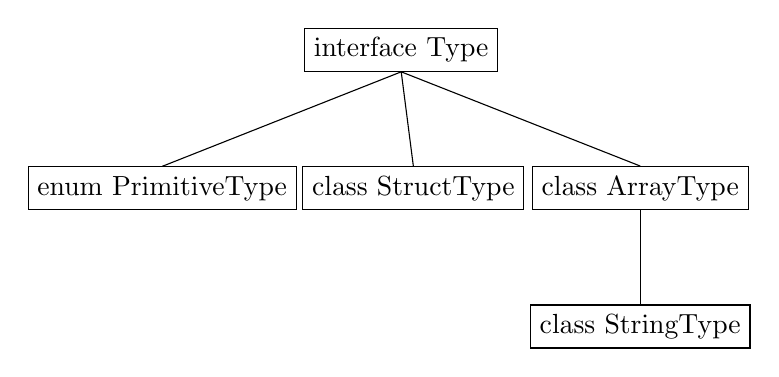
\begin{tikzpicture}
\tikzset{level distance=50pt}
\Tree [.\node[draw]{interface Type};
    [.\node[draw]{enum PrimitiveType}; ]
    [.\node[draw]{class StructType}; ]
    [.\node[draw]{class ArrayType};
        \node[draw]{class StringType};
    ]
]
\end{tikzpicture}
\end{figure}

\section{Именованные сущности (символы)}

В каждой области видимости доступна информация о всех именованных сущностях, которые доступны в ней для использования. Такие сущности называются \textit{символами} и представляются реализациями абстрактного класса \texttt{Symbol}. Всего реализация насчитывает пять видов символов: конструкторы, аргументы конструкторов, именованные типы, функции и переменные (поля структур). 

Именованные типы представлены классом \texttt{NamedType}, являющимся оберткой над \texttt{Type}, при создании экземпляра которой выполняется проверка наличия характеристики \texttt{Named} у соответствующего типа.

Функции представленны классом \texttt{Function}, экземпляры которого хранят информацию о названии, типе возвращаемого значения и списке наборов требуемых характеристик типов для каждого из аргументов.

Конструкторы представлены классом \texttt{ConstructorWithBody}, экземпляры которого хранят информацию о названии, списке аргументов (параметров) конструктора, и списке элементов конструктора. Подробнее об элементах конструкторов будет изложено позднее. Аргументы конструкторов представлены классом \texttt{ConstructorArgument}, экземпляры которого хранят информацию о названии аргумента и названии его типа, из чего следует, что типы аргументов должны быть именованными.

Переменные (поля структур) представлены классом \texttt{Variable}, экземпляры которого содержат информацию о названии, заданных на переменную ограничениях и описание переменной. Описание переменной может быть не только типом (а, например, вызовом конструктора с аргументами), об этом будет изложено позднее.

Иерархия классов реализации символов представлена на рисунке~\ref{symbol-classes-hierarchy}.

\begin{figure}[!h]
\caption{Иерархия классов реализации символов}\label{symbol-classes-hierarchy}
\centering
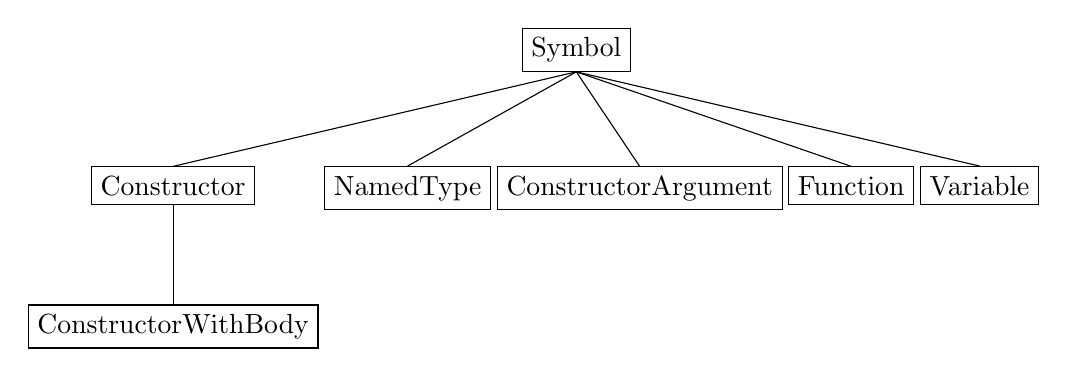
\begin{tikzpicture}
\tikzset{level distance=50pt}
\Tree [.\node[draw]{Symbol};
    [.\node[draw]{Constructor};
        \node[draw]{ConstructorWithBody};
    ]
    [.\node[draw]{NamedType}; ]
    [.\node[draw]{ConstructorArgument}; ]
    [.\node[draw]{Function}; ]
    [.\node[draw]{Variable}; ]
]
\end{tikzpicture}
\end{figure}

\section{Конструкторы}

Конструктором называется объект, ассоциированный с заданной пользователем именованной структурой и содержит информацию о названии конструктора (всегда совпадает с соответствующим типом), списке аргументов и списке элементов конструктора. Список элементов конструктора полностью определяет последовательность считываемых переменных (полей), а так же разделители между этими переменными. Элементы конструктора представлены маркерным интерфейсом \texttt{ConstructorItem}, насчитывающим три реализации: класс \texttt{Variable}~--- переменные, перечисление \texttt{IoModifier}~--- разделитель между переменными во входных или выходных данных, и \texttt{ConstructorIfAlt}~--- часть конструктора с условием.

В текущей реализации \texttt{IoModifier} может иметь только одно значение~--- \texttt{EOLN}, обозначающее перевод строки. Без указания разделителя явно будет использоваться символ пробела.

Класс \texttt{ConstructorIfAlt} отвечает за части конструкторов, которые будут задействованы или не задействованы в зависимости от какого-либо условия. Например, при описании входных и выходных данных для задачи, в которой нужно считывать запросы различных типов с разными аргументами, пользователем будет использована конструкция языка \texttt{if}, которая затем будет транслирована в экземпляр \texttt{ConstructorIfAlt}. Экземпляры этого класса хранят информацию о выражении, на основании которого будет выполнена положительная или отрицательная часть конструкции \texttt{if} и два списка элементов конструктора: для положительного и отрицательного случаев.

Иерархия классов реализации элементов конструкторов представлена на рисунке~\ref{constructor-items-classes-hierarchy}.

\begin{figure}[!h]
\caption{Иерархия классов реализации элементов конструкторов}\label{constructor-items-classes-hierarchy}
\centering
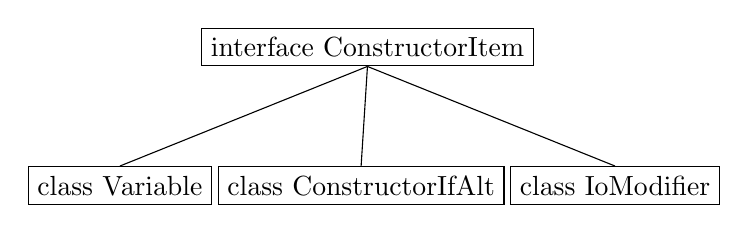
\begin{tikzpicture}
\tikzset{level distance=50pt}
\Tree [.\node[draw]{interface ConstructorItem};
    [.\node[draw]{class Variable}; ]
    [.\node[draw]{class ConstructorIfAlt}; ]
    [.\node[draw]{class IoModifier}; ]
]
\end{tikzpicture}
\end{figure}

\section{Описания переменных}

Каждый экземпляр класса \texttt{Variable} хранит в себе описание переменной~--- информацию, необходимую для генерации кода ввода или вывода этой переменной. При этом, на этапе создания экземпляров класса \texttt{Variable} типы могут быть известны не полностью. Поэтому описания переменных представлены реализациями отдельного маркерного интерфейса \texttt{VariableDescription}. При этом, любой тип может являться описанием переменной, то есть интерфейс \texttt{Type} является наследником интерфейса \texttt{VariableDescription}. Помимо этой, существует ещё три реализации описаний переменных: \texttt{NamedTypeArrayDescription}, \texttt{UnnamedStructArrayDescription} и \texttt{ParametrizedDescription}.

Классы \texttt{NamedTypeArrayDescription} и \texttt{UnnamedStructArrayDescription} отвечают за массивы именованных и неименованных типов соответственно. Каждый из них хранит в себе список параметров массива и описание типа элементов массива: экземпляр \texttt{VariableDescription} в случае именованных типов и список элементов конструктора для неименованных типов (конструкция языка описания ввода-вывода <<\texttt{array ... of}>>). Параметры массива представлены классом \texttt{ArrayParameters} и содержат в себе информацию о переменной итерирования, выражении начала итерирования, выражении окончания итерирования и списке разделителей между переменными внутри массива (список может состоять из пробелов или переводов строк).

Класс \texttt{ParametrizedDescription} в некотором смысле <<расширяет>> интерфейс \texttt{Type}, храня дополнительно список выражений, которые будут вычислены и подставлены при вызове конструктора соответствующего типа.

Иерархия классов реализации описания переменных представлена на рисунке~\ref{descriptions-classes-hierarchy}.

\begin{figure}[!h]
\caption{Иерархия классов реализации описания переменных}\label{descriptions-classes-hierarchy}
\centering
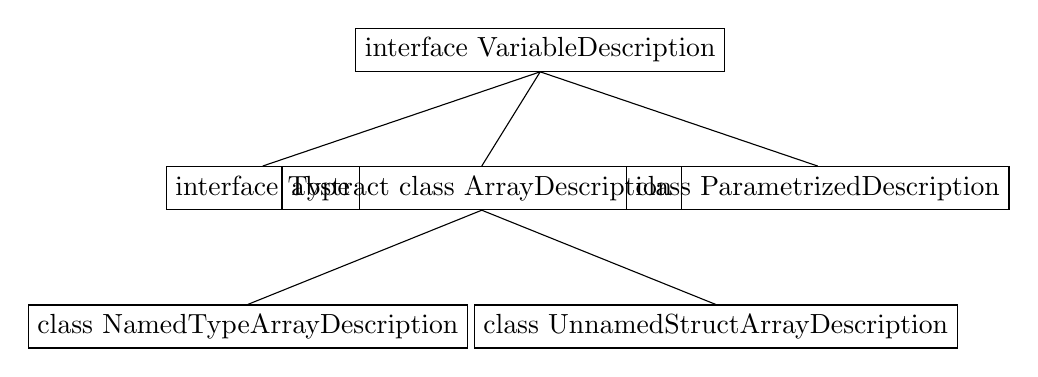
\begin{tikzpicture}
\tikzset{level distance=50pt}
\tikzset{level 1/.style={sibling distance=-120pt}}
\Tree [.\node[draw]{interface VariableDescription};
    [.\node[draw]{interface Type}; ]
    [.\node[draw]{abstract class ArrayDescription}; 
        \node[draw]{class NamedTypeArrayDescription}; 
        \node[draw]{class UnnamedStructArrayDescription}; 
    ]
    [.\node[draw]{class ParametrizedDescription}; ]
]
\end{tikzpicture}
\end{figure}

\section{Язык записи выражений}

При записи вычислимых выражений (например, при указании границ переменной итерирования при объявлении массивов и при записи логических ограничений на переменные) используется специальная часть языка описания выходных и выходных данных~--- язык выражений. Под выражением понимается языковая конструкция, которая может быть вычислена и определяет некоторое значение~\cite{mitchell2003concepts}. Синтаксис языка выражений представлен в предыдущей главе, листинге~\ref{appendix-grammar-pl-src} и в таблице~\ref{pl-operators-priority}. Здесь же будет приведено описание реализации.

Любое выражение транслируется в экземпляр какого-либо наследника базового класса \texttt{PlExpression}. Всего таких наследников существует семь:

\begin{enumerate}
    \item \texttt{PlValue}~--- литерал (константа). Хранит фиксированное значение и его тип.
    \item \texttt{PlVarBinding}~--- связывание переменной. Хранит ссылку на переменную (поле структуры), которое будет подставлено по значению в выражение и вспомогательную информацию о месте связывания.
    \item \texttt{PlSubscript}~--- представление оператора взятия элемента массива по индексу. Хранит два выражения: выражение, возвращающее массив и выражение, возвращающее необходимый индекс.
    \item \texttt{PlFunctionCall}~--- оператор вызова функции. Хранит ссылку на вызываемую функцию и список выражений аргументов функции.
    \item \texttt{PlIfOperator}~--- тернарный условный оператор. Хранит три выражения: логическое, на основании которого будет выбираться какое из последующих выражений будет возвращено в качестве результата, выражение для положительного случая и выражение для отрицательного случая.
    \item \texttt{PlUnaryOperator}~--- унарный оператор. Всего представлено три унарных оператора: логическое отрицание (требует наличие характеристики \texttt{Bool} у аргумента), побитовое отрицание (требует наличие характеристики \texttt{Integer}) и унарный минус (требует \texttt{Numeric}).
    \item \texttt{PlBinaryOperator}~--- бинарный оператор. Всего представлено девятнадцать бинарных операторов. Все бинарные операторы представлены в таблице~\ref{pl-operators-priority}.
\end{enumerate}

Каждый бинарный оператор хранит в себе список выражений~--- его аргументов. Операторы <<больше>>, <<меньше>>, <<больше или равно>> и <<меньше или равно>> не имеют ассоциативности, оператор возведения в степень имеет правую ассоциативность, остальные операторы~--- левую. Операторы <<больше>>, <<меньше>>, <<больше или равно>> и <<меньше или равно>> требуют наличие характеристики \texttt{Comparable} у типов их аргументов, операторы умножения, деления, сложения, вычитания и возведения в степень требуют наличие характеристики \texttt{Numeric}, операторы взятия остатка от деления, побитовые <<И>>, <<ИЛИ>> и <<исключающее ИЛИ>>, и операторы битовых сдвигов требуют наличия характеристики \texttt{Integer}. Операторы сравнения на равенство и не равенство требуют наличия характеристики \texttt{Can equal}. Логические операторы требуют \texttt{Bool}.

Полная иерархия классов реализации языка выражений представлена на рисунке~\ref{pl-classes-hierarchy}.

\section{Внутреннее представление}

После выполнения лексического и синтаксического разбора составляется глобальная область видимости~--- специальный экземпляр класса \texttt{Scope}, содержащий, в том числе, информацию об именах всех объявленных пользователем структур. Эта информация получается обходом дерева разбора до глубины, достаточной, чтобы зарегистрировать имя каждой структуры. Реализация этого обхода выполнена с использованием стандартного шаблона проектирования <<Посетитель>>~\cite{design-patterns}. ANTLR предоставляет стандартный интерфейс для реализации этого шаблона проектирования. Реализация представленна классом \texttt{FindGlobalSymbolsVisitor}.

Затем происходит полный обход дерева разбора описания ввода-вывода, во время которого происходит непосредственно создание экземпляров внутреннего представления, описанных выше. Реализация обхода представленна классом \texttt{ResolveSymbolsVisitor}. Сначала происходит обход поддерева, отвечающего за структуру входных данных (\texttt{input}), затем~--- обход остального дерева. Это нужно для поддержания корректности областей видимости, например, чтобы из выходных данных можно было ссылаться на переменные во входных данных.

Для каждого поддерева, отвечающего целиком за объявленную пользователем структуру, создается экземпляр конструктора, в который помещается описание структуры. При этом соответствующий структуре тип уже существует в глобальной области видимости, так как создан на предыдущем этапе обработки.

Области видимости могут <<вкладываться>> друг в друга, образуя структуру данных <<стек>>. Помимо стека областей видимости поддерживается стек названий структур и переменных итерирования для того, чтобы для каждой переменной можно было точно указать её местонахождение в иерархии структур. Кроме того, для каждого символа поддерживается список символов, от которых он зависит, то есть, список используемых им символов. Таким образом получается ациклический ориентированный граф зависимостей символов.

При обходе вершины, отвечающей за описание переменной происходит проверка, что ещё не было объявлено переменной с таким же именем, обновляется текущий путь в иерархии структур. Затем происходит обход поддерева, отвечающего за описание переменной, после чего переменная помещается в текущую область видимости. Если переменная является массивом, то выполняется обход поддерева с описанием массива. Если переменная имеет выражение-ограничение, то так же выполняется обход соответствующего поддерева.

Если описание переменной является массивом неименованной структуры, создается новая область видимости для внутренней структуры массива и выполняется обход параметров массива и непосредственно внутренней структуры. Иначе, описание переменной содержит именованный тип, проверяется его наличие в текущей области видимости. Если описание содержит аргументы конструктора, то выполняется проверка, что тип, соответствующий конструктору имеет характеристику \texttt{Parametrized}. При обходе описаний массивов в любом случае создается новая область видимости, чтобы сделать доступными для использования переменные итерирования.

При обходе вершины, отвечающей за конструкцию \texttt{if} выполняется обход поддерева с логическим выражением и обходы положительной и отрицательной веток синтаксической конструкции. Каждая ветка при этом трактуется как отдельная неименованная структура с созданием соответствующей области видимости.

Обход поддеревьев, отвечающих за выражения осуществляется экземплярами класса \texttt{PlExpressionBuildVisitor}. Его устройство тривиально, потому что он решает стандартную задачу перевода дерева разбора в абстрактное синтаксическое дерево выражения.

\chapter{Кодогенерация и интеграция в систему подготовки задач <<Polygon>>}

В этой главе описывается процесс генерации исходных кодов чекера, валидатора и грейдеров, а так же интеграция решения в систему подготовки задач по спортивному программированию <<Polygon>> и тестирование решения.

\section{Кодогенерация}

Последним этапом обработки языка описания входных и выходных данных является непосредственно генерация программных компонентов задачи. Текущая реализация может генерировать: валидаторы и чекеры с использованием библиотеки \texttt{testlib.h}~\cite{cf-testlib} на языке программирования C++, а так же грейдеры и заготовки решений на языках программирования C++, Python и Java. Эти языки были выбраны как наиболее популярные на платформе Codeforces.

Для генерации кода достаточно получить содержимое глобальной области видимости, которое описано в предыдущей главе~--- объекты в ней содержат всю необходимую информацию. Так же, на этом этапе не требуется никаких дополнительных проверок, так как они выполнены на предыдущих этапах обработки.

Вне зависимости от целевого языка программирования или компонента, генерация кода состоит из нескольких этапов:

\begin{enumerate}
    \item Генерация объявлений структур,
    \item Генерация кода ввода,
    \item Генерация кода вывода (при необходимости),
    \item Подстановка сгенерированного кода в шаблон, в котором содержатся необходимые стандартные определения, точка входа (при необходимости), вызовы чтения выходных данных, записи выходных данных и т.д.
\end{enumerate}

Генерация кода происходит построчно, то есть, во время генерации составляются списки сгенерированных строк, которые затем будут транслированы в полноценный файл с исходным кодом. Такой подход выбран для того, чтобы можно было обеспечить форматирование сгенерированного кода и сделать его <<человекочитаемым>>.

\subsection{Генерация объявлений структур}

Генерация объявлений структур происходит следующим образом. Поочередно перебираются все конструкторы в глобальной области видимости, то есть все объявленные пользователем структуры, в порядке топологической сортировки графа зависимостей символов. Таким образом, в сгенерированном коде структуры находятся строго после всех необходимых объявлений, то есть зависимости направлены сверху вниз. Направление зависимостей в исходном коде критично для таких языков программирования как C++~\cite{cppbook}.

Для генерации объявления каждой конкретной структуры происходит обход списка всех элементов конструктора за исключением модификаторов ввода-вывода, так как они не влияют на представление данных. Переменные транслируются тривиальным, зависимым от целевого языка программирования, образом~--- в сгенерированном коде объявляется соответствующее поле структуры (или класса) с соответствующим типом. Условные конструкции (\texttt{if}) <<схлопываются>> в <<плоскую>> структуру, то есть поля, объявленные в разных ветках будут транслироваться непосредственно в поля внешней структуры или класса.

Для массивов неименованных структур генерируются структуры или классы с названиями, соответствующими названиям переменных, поэтому процесс генерации кода определений для них не отличается от процесса генерации кода определений для именованных структур.

Реализации генерации объявлений структур для языков программирования C++, Java и Python представлены классами \texttt{CppStructDeclarationsTranslator}, \texttt{JavaStructDeclarationsTranslator} и \texttt{PythonStructDeclarationsTranslator} соответственно. В случае C++ генерируется набор структур (\texttt{struct}), в случаях Java и Python генерируется набор классов (\texttt{class}).

\subsection{Генерация выражений}

Код для ввода и вывода может использовать выражения, например, при определении интервалов переменных итерирования или для проверки логических условий на переменные. Генерация кода выражений, для простоты реализации, выделена в отдельные классы: \texttt{CppPlExpressionTranslator}, \texttt{JavaPlExpressionTranslator} и \texttt{PythonPlExpressionTranslator} для языков программирования C++, Java и Python соответственно.

Для того, чтобы корректно провести трансляцию выражений необходимо знать местоположение выражения в описании входных и выходных данных и набор локальных переменных в текущей области видимости. Эта информация передается при создании экземпляра соответствующего класса-транслятора. Сама трансляция происходит тривиальным образом: абстрактное синтаксическое дерево выражение преобразуется в конструкции соответствующего целевого языка программирования. Если в языке программирования нет прямых аналогов нужной функциональности, происходит трансляция в вызов вспомогательной функции, реализация которой будет предоставлена в шаблоне на соответствующем языке.

\subsection{Генерация кода ввода}

Генерация кода ввода происходит следующим образом. Перебираются все конструкторы в глобальной области видимости, для каждого генерируется функция, которая будет считывать из потока ввода соответствующую структуру и возвращать её в качестве результата. При этом, если целевой язык~--- С++, то сигнатуры функций и их реализации генерируются по-отдельности, чтобы функции ссылались только на уже объявленные в коде функции.

Для каждой структуры генерируется функция считывания, которая поочередно считывает поля соответствующей структуры или класса из стандартного потока ввода. Если очередное поле является встроенным в язык описания входных и выходных данных типом, то вызывается соответствующая конструкция целевого языка для считывания из ввода. Если же очередное считываемое поле является структурой, то происходит вызов сгенерированной функции считывания соответствующей структуры.

Для считывания массивов генерируется цикл на целевом языке программирования, в теле которого происходит считывание каждого элемента массива, которые поочередно добавляются в конец массива.

При наличии в структуре, для которой генерируется код ввода, условной конструкции \texttt{if}, генерируется условная конструкция на целевом языке программирования. Генерация веток условной конструкции происходит так же, как и генерация самих структур.

Для целевых языков программирования C++ и Java используются стандартные средства разбора потока ввода~--- \texttt{cin}~\cite{cppcin} и \texttt{Scanner}~\cite{javascanner} соответственно. Язык Python предоставляет ограниченные возможности для разбора стандартного потока ввода, поэтому, для него была написана собственная реализация разбора, которая встроена в шаблон для этого языка.

Реализация генерации кода ввода представлена классами \texttt{CppGraderReadTranslator}, \texttt{JavaGraderReadTranslator} и \texttt{PythonGraderReadTranslator}.

\subsubsection{Особенности генерации валидатора и чекера}

Генерируемый код валидатора, по своей сути, является несколько модифицированным кодом ввода структуры \texttt{input} и её зависимостей. При этом сгенерированный код использует не стандартный способ разбора входных данных, а методы семейства <<\texttt{readX(...)}>> из библиотеки \texttt{testlib.h}~\cite{cf-testlib}. 

При этом, между считыванием полей, происходит проверка, что разделитель соответствует заданному в описании ввода-вывода, вызовом метода \texttt{readSpace()} или \texttt{readEoln()}. Так же, после кода считывания каждого поля, при необходимости, вставляется код, проверяющий заданное в описании ввода-вывода логическое ограничение (вызов метода \texttt{ensuref(...)}).

В случае чекера, в каждой генерируемой функции добавляется дополнительный аргумент \texttt{InStream\& stream}~--- поток \texttt{testlib.h}, из которого будет происходить считывание. Всего в чекере существует три потока: поток входных данных, поток ответа участника и поток ответа жюри (ответа авторского решения). В чекере происходит считывание всех трёх потоков.

Реализация генерации кода валидатора и чекера представлена классами \texttt{CppTestlibValidatorTranslator} и \texttt{CppTestlibCheckerTranslator} соответственно.

\subsection{Генерация кода вывода}

Генерация кода для вывода структур происходит аналогично генерации кода для ввода за исключением того, что методы, осуществляющие вывод не возвращают структуру, а принимают её в качестве аргумента. Так же, при выводе учитываются разделители полей в структурах и, при необходимости, в код вставляются операции перевода строки. Во всех целевых языках используются стандартные конструкции для форматированного вывода данных (\texttt{cout}, \texttt{print(...)}, \texttt{PrintStream}).

Реализация генерации кода вывода представлена классами \texttt{CppGraderWriteTranslator}, \texttt{JavaGraderWriteTranslator} и \texttt{PythonGraderWriteTranslator}.

\subsection{Шаблоны}

Выше описан процесс генерации кода, зависящего от описания входных и выходных данных задачи. Однако, часть результирующего исходного кода берется из заранее написанных шаблонов. Шаблоны содержат вспомогательные определения, необходимые для работы сгенерированного кода. Например, шаблон для грейдера на языке программирования Python содержит определение вспомогательного класса \texttt{Scanner} для разбора ввода.

После подстановки сгенерированного кода в шаблон получается один или несколько полноценных файлов с исходным кодом валидатора, чекера или грейдеров. После этого автору задачи остается лишь дополнить файлы специфичной для задачи логикой.

\section{Интеграция в <<Polygon>>}

Решение было реализовано на языке программирования Java версии 17. Эта версия была выбрана как последняя стабильная с долгим циклом поддержки. Так же, использование современной версии языка программирования Java позволило сократить исходный код реализации решения за счет использования последних возможностей этого языка.

Однако, интеграция решения непосредственно в систему подготовки задач <<Polygon>> при этом оказалось затруднительной, так как исходный код <<Polygon>> написан с использованием Java версии 8. Поэтому решение было реализовано в качестве отдельного сервиса, которому <<Polygon>> при необходимости отсылает запросы на генерацию кода и в ответ получает готовые файлы.

Решение упаковывается в исполняемый jar-файл и может использоваться как в качестве отдельного сервиса, так и как утилита командной строки. Точкой входа является класс \texttt{IoMarkupCli}.

При работе в режиме утилиты командной строки, считывается файл, указанный в аргументах командной строки, на языке описания входных и выходных данных и создаются сгенерированные файлы с исходным кодом запрошенных в аргументах командной строки целевых компонент задачи на целевых языках. После этого выполнение завершается.

При запуске в режиме сервиса (демона, от англ. \textit{daemon}) слушается указанный в аргументах порт, на который будут поступать запросы. В силу особенностей существующей архитектуры системы подготовки задач по спортивному программированию <<Polygon>> протоколом обращения к сервису генерации кода, так же как и протоколом получения ответа, был выбран XML-RPC~\cite{laurent2001programming}, содержащий сериализованные данные запроса в формате Protobuf~\cite{protobufdocs}. Ответ так же содержит сериализованные данные в формате Protobuf.

\subsection{Структура запросов и ответов}

Ознакомиться с определением структуры запросов и ответов в формате Protobuf можно в приложении~\ref{appendix-protobuf}.

В запросе (\texttt{GenerateRequest}) содержится строка (поле \texttt{io\_markup})~--- описание входных и выходных данных и набор структур, описывающих целевой компонент и язык программирования для генерации кода (поле \texttt{target\_file\_description}). \texttt{TargetFileDescription} содержит целевой компонент (один из элементов перечисления \texttt{TargetComponent}) и язык генерации (один из элементов перечисления \texttt{TargetLanguage}).

В ответе (\texttt{GenerateResponse}) содержится список сгенерированных файлов в поле \texttt{result\_file} и, возможно, сообщение об ошибке в поле \texttt{error\_message}. Каждый сгенерированный файл (\texttt{ResultFile}) содержит компонент и язык программирования, название файла (поле \texttt{name}), содержимое файла в строковом виде (поле \texttt{content}) и необязательное сообщение об ошибке.

Все строки представляются в кодировке UTF-8.

\subsection{Поддержка в <<Polygon>>}

Поддержка со стороны исходного кода системы подготовки задач по спортивному программированию <<Polygon>> сводится к реализации интерфейса пользователя, отправки запросов, приема ответов и записи в репозиторий задачи сгенерированных файлов с исходным кодом. Процесс отправки запросов и приема ответов прозрачен для кода <<Polygon>> ввиду использования XML-RPC, то есть цикл <<запрос-ответ>> выглядит как один вызов удаленной процедуры. В случае наличия ошибок в ответе, они будут выданы пользователю (автору задачи).

С точки зрения пользователя процесс выглядит следующим образом. В репозитории задачи в разделе ресурсов (Files~--- Resource Files) создается специальный файл на языке описания входных и выходных данных с именем <<\texttt{iomarkup.txt}>>. В файле записывается описание ввода-вывода. В списке файлов появляется ссылка на страницу генерации (Generate). Страница со списком файлов показана на рисунке~\ref{resources-screenshot}.

\begin{figure}[!h]
\caption{Список ресурсов задачи}\label{resources-screenshot}
\centering
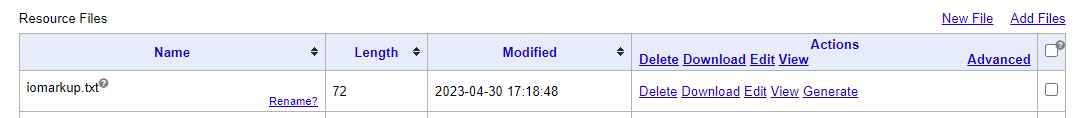
\includegraphics[scale=0.6]{img/files.png}
\end{figure}

На странице генерации пользователь выбирает какие программные компоненты нужно сгенерировать и на каких языках программирования. Страница с выбором показана на рисунке~\ref{generate-screenshot}.

\begin{figure}[!h]
\caption{Выбор параметров генерации}\label{generate-screenshot}
\centering
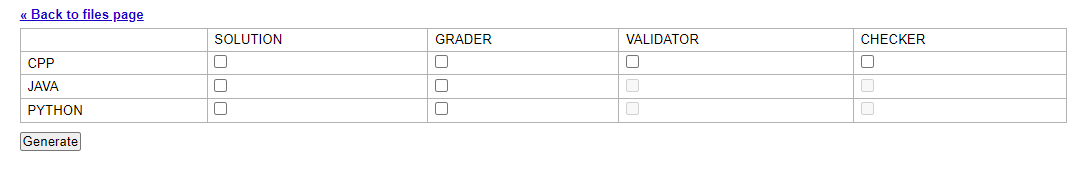
\includegraphics[scale=0.6]{img/generate.png}
\end{figure}

\subsection{Сервис кодогенерации}

В силу особенностей используемой библиотеки, реализующей протокол XML-RPC, реализация конечной точки обработки запроса на генерацию кода представлена реализацией интерфейса \texttt{com.codeforces.interop.iomarkup.InteropRpc} классом \texttt{InteropRpcImpl}. При получении запроса, происходит десериализация тела запроса на генерацию из массива байт, затем обработка запроса по алгоритмам, описанным выше в работе и сериализация ответа с помощью Protobuf в массив байт. При возникновении ошибки обработка прекращается и ответ, содержащий описание ошибки, возвращается немедленно.

\section{Тестирование}

Тестирование предложенного в данной работе решения производилось на нескольких соревнованиях на платформе Codeforces. Для задач соревнований были вручную написаны описания входных и выходных данных и сгенерированны валидатор, чекер и грейдеры. Для каждого сгенерированного компонента на каждом языке проверялось, что сгенерированный код компилируется без ошибок (в случае Python проверялась корректности синтаксиса).

Рассмотрим множество всех возможных файлов. Валидатор для задачи должен выдавать положительный результат (вердикт <<Корректный тест>>) на подмножестве этого множества. При этом, сгенерированный валидатор должен выдавать положительный результат для подмножества множества всех возможных файлов, но, для надмножества множества корректных тестов, определяемых <<настоящим>> валидатором. Иными словами, не должно быть такого файла, для которого <<настоящий валидатор>> выдаст вердикт <<Корректный тест>>, а сгенерированный~--- <<Некорректный тест>>.

Для каждой задачи при тестировании автоматически загружался пакет задачи из <<Polygon>>. Для каждого теста валидатора, для которого валидатор из пакета задачи выдавал вердикт <<Корректный тест>> проверялось, что сгенерированный валидатор выдавал такой же вердикт. Для всех наборов входных данных из пакета задачи проверялось, что сгенерированный валидатор выдает вердикт <<Корректный тест>> на каждом из них. 

Тестирование происходило в условиях, максимально приближенных к тем, в которых происходит тестирование на платформах <<Codeforces>> и <<Polygon>>. Для этого проект <<Invoker>>, который реализует полный цикл тестирования на вышеупомянутых платформах, был подготовлен для использования в качестве отдельной библиотеки и добавлен в качестве тестовой зависимости в реализацию решения в данной работе.

\startconclusionpage

В данной работе был спроектирован язык описания входных и выходных данных для задач по программированию, позволяющий описывать их структуру и формат. Реализована и описана система частичной генерации исходных кодов валидатора, чекера и грейдеров, включающих в себя реализацию ввода-вывода данных, описание структур, необходимых в задаче, а так же проверку логических условий, заданных автором. Полученная система интегрированна в сервис для подготовки задач по спортивному программированию <<Polygon>>, на работу получен акт о внедрении.

\printmainbibliography

\appendix

\chapter{Грамматика языка описания}\label{appendix-antlr-grammar}

\begin{lstlisting}[
    caption={Определения токенов в формате ANTLR 4},
    keywordstyle=\color{black},
    commentstyle=\color{black},
    stringstyle=\color{black},
    label={appendix-lexer-src}
]
LINE_COMMENT: '#' .*? '\r'? ('\n' | EOF) -> skip;
COMMENT: '/*' .*? '*/' -> skip;

fragment ESCAPED_CHAR: '\\n';

CHAR: '\'' ((~['\\\r\n]) | ESCAPED_CHAR) '\'';
STRING: '"' ((~["\\\r\n]) | ESCAPED_CHAR)* '"';
TRUE: 'true';
FALSE: 'false';
LOGICAL_AND: '&&';
LOGICAL_OR: '||';
LOGICAL_NOT: '!';
BITWISE_AND: '&';
BITWISE_XOR: '^';
PIPE: '|';
BITWISE_NOT: '~';
EQUALS: '==';
NOT_EQUALS: '!=';
LESS_EQUAL: '<=';
GREATER_EQUAL: '>=';
LESS: '<';
GREATER: '>';
PLUS: '+';
MINUS: '-';
POW: '**';
MULTIPLICATION: '*';
DIVISION: '/';
MODULO: '%';
DOT: '.';
COLON: ':';
QUESTION: '?';
ASSIGN: '=';
COMMA: ',';
SEMICOLON: ';';
LBRACE: '{';
RBRACE: '}';
LBRACKET: '[';
RBRACKET: ']';
LPAR: '(';
RPAR: ')';
SEP: 'sep';
EOLN_MODIFIER: 'eoln';
IF: 'if';
ARRAY: 'array';
OF: 'of';
ELSE: 'else';

fragment U_NUM_LITERAL_MODIFIER: 'u' | 'U';
fragment L_NUM_LITERAL_MODIFIER: 'l' | 'L';
fragment F_NUM_LITERAL_MODIFIER: 'f' | 'F';
fragment EXPONENT: 'e' | 'E';
fragment DIGITS: [0-9][0-9'_]*;

fragment INTEGER_SUFFIX: U_NUM_LITERAL_MODIFIER? L_NUM_LITERAL_MODIFIER?;
fragment FLOAT_SUFFIX: ('.' DIGITS)? (EXPONENT DIGITS)? F_NUM_LITERAL_MODIFIER?;

NUM_VALUE: DIGITS INTEGER_SUFFIX FLOAT_SUFFIX;

NAME: [a-zA-Z_][a-zA-Z0-9_]*;
WS: [ \t\r\n]+ -> skip;
\end{lstlisting}

\begin{lstlisting}[
    caption={Грамматика языка описания в формате ANTLR 4},
    keywordstyle=\color{black},
    commentstyle=\color{black},
    stringstyle=\color{black},
    label={appendix-grammar-src}
]
ioMarkup: (namedStruct)* EOF;
namedStruct: NAME namedStructParameters? struct;
namedStructParameters: LPAR (parameterDeclaration (COMMA parameterDeclaration)*)? RPAR;
parameterDeclaration: NAME COLON namedType;
struct: LBRACE structItem* RBRACE;
structItem: conditionalAlternative | variableDeclaration | ioModifier;
conditionalAlternative: IF LPAR plExpression RPAR struct (ELSE struct)?;
ioModifier: EOLN_MODIFIER SEMICOLON;
variableDeclaration: NAME COLON variableType variableConstraint? SEMICOLON;
variableType: arrayOfUnnamedStruct | (namedType namedTypeParameters? arrayParameters*);
arrayOfUnnamedStruct: ARRAY arrayParameters+ OF struct;
variableConstraint: PIPE plExpression;
namedType: NAME;
namedTypeParameters: LPAR (plExpression (COMMA plExpression)*)? RPAR;
arrayParameters: LBRACKET arrayIterationRange (COMMA SEP ASSIGN sepValue) RBRACKET;
arrayIterationRange: NAME ASSIGN plExpression DOT DOT plExpression;
sepValue: STRING | CHAR;
\end{lstlisting}

\begin{lstlisting}[
    caption={Грамматика языка выражений в формате ANTLR 4},
    keywordstyle=\color{black},
    commentstyle=\color{black},
    stringstyle=\color{black},
    label={appendix-grammar-pl-src}
]
plExpression: plImplLogicalOr (QUESTION plImplLogicalOr COLON plImplLogicalOr)?;

plImplLogicalOr: plImplLogicalAnd (LOGICAL_OR plImplLogicalAnd)*;
plImplLogicalAnd: plImplBitwiseOr (LOGICAL_AND plImplBitwiseOr)*;
plImplBitwiseOr: plImplBitwiseXor (PIPE plImplBitwiseXor)*;
plImplBitwiseXor: plImplBitwiseAnd (BITWISE_XOR plImplBitwiseAnd)*;
plImplBitwiseAnd: plImplEquality (BITWISE_AND plImplEquality)*;
plImplEquality: plImplRelational (plImplEqualityOp plImplRelational)*;
plImplRelational: plImplBitwiseShift (plImplRelationalOp plImplBitwiseShift)?;
plImplBitwiseShift: plImplAdditiveBinary (plImplBitwiseShiftOp plImplAdditiveBinary)?;
plImplAdditiveBinary: plImplMultiplicativeBinary (plImplAdditiveOp plImplMultiplicativeBinary)*;
plImplMultiplicativeBinary: plImplPowBinary (plImplMultiplicativeBinaryOp plImplPowBinary)*;
plImplPowBinary: plImplPrefixUnary (POW plImplPrefixUnary)*;
plImplPrefixUnary: plImplPrefixUnaryOp* plImplHighestPriority;

plImplHighestPriority: ((LPAR plExpression RPAR) | plFunctionCall | plValue | plVarBinding) plSubscript*;

plImplEqualityOp: EQUALS | NOT_EQUALS;
plImplRelationalOp: GREATER | LESS | GREATER_EQUAL | LESS_EQUAL;
plImplAdditiveOp: PLUS | MINUS;
plImplMultiplicativeBinaryOp: MULTIPLICATION | DIVISION | MODULO;
plImplPrefixUnaryOp: LOGICAL_NOT | BITWISE_NOT | MINUS;
plImplBitwiseShiftOp: LESS LESS | GREATER GREATER;

plFunctionCall: NAME LPAR plImplFunctionArgs? RPAR;
plImplFunctionArgs: plExpression (COMMA plExpression)*;

plVarBinding: NAME;

plSubscript: LBRACKET plExpression RBRACKET;

plValue: plNumValue | plBoolValue | plCharValue | plStringValue;
plBoolValue: TRUE | FALSE;
plCharValue: CHAR;
plStringValue: STRING;
plNumValue: NUM_VALUE;
\end{lstlisting}

\chapter{Язык записи выражений}\label{appendix-pl-operators-priority}

\begin{table}[!h]
\caption{Операторы языка выражений в порядке уменьшения приоритета}\label{pl-operators-priority}
\centering
\begin{adjustbox}{angle=-90}
\begin{tabular}{|*{4}{c|}}\hline
Приоритет & Нетерминал & Оператор & Описание\\\hline
1  & \texttt{plImplHighestPriority} & \texttt{f(x)} & Вызов функции \\\hline
1  & \texttt{plImplHighestPriority} & \texttt{x[y]} & Взятие по индексу \\\hline
2  & \texttt{plImplPrefixUnary} & \texttt{!x} & Логическое отрицание \\\hline
2  & \texttt{plImplPrefixUnary} & \texttt{~x} & Инверсия битов \\\hline
2  & \texttt{plImplPrefixUnary} & \texttt{-x} & Унарный минус \\\hline
3  & \texttt{plImplPowBinary} & \texttt{x ** y} & Возведение в степень \\\hline
4  & \texttt{plImplMultiplicativeBinary} & \texttt{x * y} & Умножение \\\hline
4  & \texttt{plImplMultiplicativeBinary} & \texttt{x / y} & Деление \\\hline
4  & \texttt{plImplMultiplicativeBinary} & \texttt{x \% y} & Остаток от деления \\\hline
5  & \texttt{plImplAdditiveBinary} & \texttt{x + y} & Сложение \\\hline
5  & \texttt{plImplAdditiveBinary} & \texttt{x - y} & Вычитание \\\hline
6  & \texttt{plImplBitwiseShift} & \texttt{x >{>} y} & Побитовый сдвиг вправо \\\hline
6  & \texttt{plImplBitwiseShift} & \texttt{x <{<} y} & Побитовый сдвиг влево \\\hline
7  & \texttt{plImplRelationalOp} & \texttt{>}, \texttt{<}, \texttt{>=}, \texttt{<=} & Сравнение \\\hline
8  & \texttt{plImplEquality} & \texttt{x == y} & Равенство \\\hline
8  & \texttt{plImplEquality} & \texttt{x != y} & Неравенство \\\hline
9  & \texttt{plImplBitwiseAnd} & \texttt{x \& y} & Побитовое <<И>> \\\hline
10  & \texttt{plImplBitwiseXor}  & \texttt{x \textasciicircum~y} & Побитовое исключающее <<ИЛИ>> \\\hline
11  & \texttt{plImplBitwiseOr}  & \texttt{x | y} & Побитовое <<ИЛИ>> \\\hline
12  & \texttt{plImplLogicalAnd}  & \texttt{x \&\& y} & Конъюнкция \\\hline
13  & \texttt{plImplLogicalOr}  & \texttt{x || y} & Дизъюнкция \\\hline
14  & \texttt{plExpression}  & \texttt{x ? y : x} & Тернарный условный оператор \\\hline
\end{tabular}
\end{adjustbox}
\end{table}

\begin{figure}[!h]
\caption{Иерархия классов реализации языка выражений}\label{pl-classes-hierarchy}
\centering
\begin{adjustbox}{angle=-90}
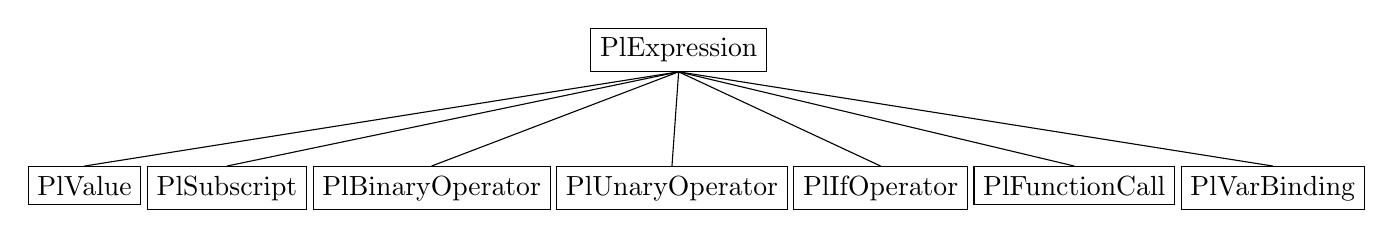
\begin{tikzpicture}
\tikzset{level distance=50pt}
\Tree [.\node[draw]{PlExpression};
    [.\node[draw]{PlValue}; ]
    [.\node[draw]{PlSubscript}; ]
    [.\node[draw]{PlBinaryOperator}; ]
    [.\node[draw]{PlUnaryOperator}; ]
    [.\node[draw]{PlIfOperator}; ]
    [.\node[draw]{PlFunctionCall}; ]
    [.\node[draw]{PlVarBinding}; ]
]
\end{tikzpicture}
\end{adjustbox}
\end{figure}


\chapter{Структура запросов и ответов сервиса генерации}\label{appendix-protobuf}

\begin{lstlisting}[
    caption={Структура запросов и ответов сервиса генерации в формате Protobuf},
    keywordstyle=\color{black},
    commentstyle=\color{black},
    stringstyle=\color{black},
    label={appendix-protobuf-src}
]
syntax = "proto2";

enum TargetLanguage {
    CPP = 0;
    JAVA = 1;
    PYTHON = 2;
}
enum TargetComponent {
    SOLUTION = 0;
    GRADER = 1;
    VALIDATOR = 2;
    CHECKER = 3;
}
message TargetFileDescription {
    required TargetComponent target_component = 1;
    required TargetLanguage target_language = 2;
    optional string name = 3;
    optional string previous_content = 4;
}
message ResultFile {
    required TargetComponent component = 1;
    required TargetLanguage language = 2;
    required string name = 3;
    required string content = 4;
    optional string error_message = 5;
}
message GenerateRequest {
    required string io_markup = 1;
    repeated TargetFileDescription target_file_description = 2;
}
message GenerateResponse {
    repeated ResultFile result_file = 1;
    optional string error_message = 2;
}
\end{lstlisting}

\end{document}
